
%% bare_jrnl.tex
%% V1.4b
%% 2015/08/26
%% by Michael Shell
%% see http://www.michaelshell.org/
%% for current contact information.
%%
%% This is a skeleton file demonstrating the use of IEEEtran.cls
%% (requires IEEEtran.cls version 1.8b or later) with an IEEE
%% journal paper.
%%
%% Support sites:
%% http://www.michaelshell.org/tex/ieeetran/
%% http://www.ctan.org/pkg/ieeetran
%% and
%% http://www.ieee.org/

%%*************************************************************************
%% Legal Notice:
%% This code is offered as-is without any warranty either expressed or
%% implied; without even the implied warranty of MERCHANTABILITY or
%% FITNESS FOR A PARTICULAR PURPOSE! 
%% User assumes all risk.
%% In no event shall the IEEE or any contributor to this code be liable for
%% any damages or losses, including, but not limited to, incidental,
%% consequential, or any other damages, resulting from the use or misuse
%% of any information contained here.
%%
%% All comments are the opinions of their respective authors and are not
%% necessarily endorsed by the IEEE.
%%
%% This work is distributed under the LaTeX Project Public License (LPPL)
%% ( http://www.latex-project.org/ ) version 1.3, and may be freely used,
%% distributed and modified. A copy of the LPPL, version 1.3, is included
%% in the base LaTeX documentation of all distributions of LaTeX released
%% 2003/12/01 or later.
%% Retain all contribution notices and credits.
%% ** Modified files should be clearly indicated as such, including  **
%% ** renaming them and changing author support contact information. **
%%*************************************************************************


% *** Authors should verify (and, if needed, correct) their LaTeX system  ***
% *** with the testflow diagnostic prior to trusting their LaTeX platform ***
% *** with production work. The IEEE's font choices and paper sizes can   ***
% *** trigger bugs that do not appear when using other class files.       ***                          ***
% The testflow support page is at:
% http://www.michaelshell.org/tex/testflow/



\documentclass[journal]{IEEEtran}
\usepackage{graphicx}
\usepackage{cite}
\usepackage{amsmath}
\usepackage{float}
\usepackage{wrapfig}
\usepackage{subfig}
%
% If IEEEtran.cls has not been installed into the LaTeX system files,
% manually specify the path to it like:
% \documentclass[journal]{../sty/IEEEtran}





% Some very useful LaTeX packages include:
% (uncomment the ones you want to load)


% *** MISC UTILITY PACKAGES ***
%
%\usepackage{ifpdf}
% Heiko Oberdiek's ifpdf.sty is very useful if you need conditional
% compilation based on whether the output is pdf or dvi.
% usage:
% \ifpdf
%   % pdf code
% \else
%   % dvi code
% \fi
% The latest version of ifpdf.sty can be obtained from:
% http://www.ctan.org/pkg/ifpdf
% Also, note that IEEEtran.cls V1.7 and later provides a builtin
% \ifCLASSINFOpdf conditional that works the same way.
% When switching from latex to pdflatex and vice-versa, the compiler may
% have to be run twice to clear warning/error messages.






% *** CITATION PACKAGES ***
%
%\usepackage{cite}
% cite.sty was written by Donald Arseneau
% V1.6 and later of IEEEtran pre-defines the format of the cite.sty package
% \cite{} output to follow that of the IEEE. Loading the cite package will
% result in citation numbers being automatically sorted and properly
% "compressed/ranged". e.g., [1], [9], [2], [7], [5], [6] without using
% cite.sty will become [1], [2], [5]--[7], [9] using cite.sty. cite.sty's
% \cite will automatically add leading space, if needed. Use cite.sty's
% noadjust option (cite.sty V3.8 and later) if you want to turn this off
% such as if a citation ever needs to be enclosed in parenthesis.
% cite.sty is already installed on most LaTeX systems. Be sure and use
% version 5.0 (2009-03-20) and later if using hyperref.sty.
% The latest version can be obtained at:
% http://www.ctan.org/pkg/cite
% The documentation is contained in the cite.sty file itself.






% *** GRAPHICS RELATED PACKAGES ***
%
\ifCLASSINFOpdf
  % \usepackage[pdftex]{graphicx}
  % declare the path(s) where your graphic files are
  % \graphicspath{{../pdf/}{../jpeg/}}
  % and their extensions so you won't have to specify these with
  % every instance of \includegraphics
  % \DeclareGraphicsExtensions{.pdf,.jpeg,.png}
\else
  % or other class option (dvipsone, dvipdf, if not using dvips). graphicx
  % will default to the driver specified in the system graphics.cfg if no
  % driver is specified.
  % \usepackage[dvips]{graphicx}
  % declare the path(s) where your graphic files are
  % \graphicspath{{../eps/}}
  % and their extensions so you won't have to specify these with
  % every instance of \includegraphics
  % \DeclareGraphicsExtensions{.eps}
\fi
% graphicx was written by David Carlisle and Sebastian Rahtz. It is
% required if you want graphics, photos, etc. graphicx.sty is already
% installed on most LaTeX systems. The latest version and documentation
% can be obtained at: 
% http://www.ctan.org/pkg/graphicx
% Another good source of documentation is "Using Imported Graphics in
% LaTeX2e" by Keith Reckdahl which can be found at:
% http://www.ctan.org/pkg/epslatex
%
% latex, and pdflatex in dvi mode, support graphics in encapsulated
% postscript (.eps) format. pdflatex in pdf mode supports graphics
% in .pdf, .jpeg, .png and .mps (metapost) formats. Users should ensure
% that all non-photo figures use a vector format (.eps, .pdf, .mps) and
% not a bitmapped formats (.jpeg, .png). The IEEE frowns on bitmapped formats
% which can result in "jaggedy"/blurry rendering of lines and letters as
% well as large increases in file sizes.
%
% You can find documentation about the pdfTeX application at:
% http://www.tug.org/applications/pdftex





% *** MATH PACKAGES ***
%
%\usepackage{amsmath}
% A popular package from the American Mathematical Society that provides
% many useful and powerful commands for dealing with mathematics.
%
% Note that the amsmath package sets \interdisplaylinepenalty to 10000
% thus preventing page breaks from occurring within multiline equations. Use:
%\interdisplaylinepenalty=2500
% after loading amsmath to restore such page breaks as IEEEtran.cls normally
% does. amsmath.sty is already installed on most LaTeX systems. The latest
% version and documentation can be obtained at:
% http://www.ctan.org/pkg/amsmath





% *** SPECIALIZED LIST PACKAGES ***
%
%\usepackage{algorithmic}
% algorithmic.sty was written by Peter Williams and Rogerio Brito.
% This package provides an algorithmic environment fo describing algorithms.
% You can use the algorithmic environment in-text or within a figure
% environment to provide for a floating algorithm. Do NOT use the algorithm
% floating environment provided by algorithm.sty (by the same authors) or
% algorithm2e.sty (by Christophe Fiorio) as the IEEE does not use dedicated
% algorithm float types and packages that provide these will not provide
% correct IEEE style captions. The latest version and documentation of
% algorithmic.sty can be obtained at:
% http://www.ctan.org/pkg/algorithms
% Also of interest may be the (relatively newer and more customizable)
% algorithmicx.sty package by Szasz Janos:
% http://www.ctan.org/pkg/algorithmicx




% *** ALIGNMENT PACKAGES ***
%
%\usepackage{array}
% Frank Mittelbach's and David Carlisle's array.sty patches and improves
% the standard LaTeX2e array and tabular environments to provide better
% appearance and additional user controls. As the default LaTeX2e table
% generation code is lacking to the point of almost being broken with
% respect to the quality of the end results, all users are strongly
% advised to use an enhanced (at the very least that provided by array.sty)
% set of table tools. array.sty is already installed on most systems. The
% latest version and documentation can be obtained at:
% http://www.ctan.org/pkg/array


% IEEEtran contains the IEEEeqnarray family of commands that can be used to
% generate multiline equations as well as matrices, tables, etc., of high
% quality.




% *** SUBFIGURE PACKAGES ***
%\ifCLASSOPTIONcompsoc
%  \usepackage[caption=false,font=normalsize,labelfont=sf,textfont=sf]{subfig}
%\else
%  \usepackage[caption=false,font=footnotesize]{subfig}
%\fi
% subfig.sty, written by Steven Douglas Cochran, is the modern replacement
% for subfigure.sty, the latter of which is no longer maintained and is
% incompatible with some LaTeX packages including fixltx2e. However,
% subfig.sty requires and automatically loads Axel Sommerfeldt's caption.sty
% which will override IEEEtran.cls' handling of captions and this will result
% in non-IEEE style figure/table captions. To prevent this problem, be sure
% and invoke subfig.sty's "caption=false" package option (available since
% subfig.sty version 1.3, 2005/06/28) as this is will preserve IEEEtran.cls
% handling of captions.
% Note that the Computer Society format requires a larger sans serif font
% than the serif footnote size font used in traditional IEEE formatting
% and thus the need to invoke different subfig.sty package options depending
% on whether compsoc mode has been enabled.
%
% The latest version and documentation of subfig.sty can be obtained at:
% http://www.ctan.org/pkg/subfig




% *** FLOAT PACKAGES ***
%
%\usepackage{fixltx2e}
% fixltx2e, the successor to the earlier fix2col.sty, was written by
% Frank Mittelbach and David Carlisle. This package corrects a few problems
% in the LaTeX2e kernel, the most notable of which is that in current
% LaTeX2e releases, the ordering of single and double column floats is not
% guaranteed to be preserved. Thus, an unpatched LaTeX2e can allow a
% single column figure to be placed prior to an earlier double column
% figure.
% Be aware that LaTeX2e kernels dated 2015 and later have fixltx2e.sty's
% corrections already built into the system in which case a warning will
% be issued if an attempt is made to load fixltx2e.sty as it is no longer
% needed.
% The latest version and documentation can be found at:
% http://www.ctan.org/pkg/fixltx2e


%\usepackage{stfloats}
% stfloats.sty was written by Sigitas Tolusis. This package gives LaTeX2e
% the ability to do double column floats at the bottom of the page as well
% as the top. (e.g., "\begin{figure*}[!b]" is not normally possible in
% LaTeX2e). It also provides a command:
%\fnbelowfloat
% to enable the placement of footnotes below bottom floats (the standard
% LaTeX2e kernel puts them above bottom floats). This is an invasive package
% which rewrites many portions of the LaTeX2e float routines. It may not work
% with other packages that modify the LaTeX2e float routines. The latest
% version and documentation can be obtained at:
% http://www.ctan.org/pkg/stfloats
% Do not use the stfloats baselinefloat ability as the IEEE does not allow
% \baselineskip to stretch. Authors submitting work to the IEEE should note
% that the IEEE rarely uses double column equations and that authors should try
% to avoid such use. Do not be tempted to use the cuted.sty or midfloat.sty
% packages (also by Sigitas Tolusis) as the IEEE does not format its papers in
% such ways.
% Do not attempt to use stfloats with fixltx2e as they are incompatible.
% Instead, use Morten Hogholm'a dblfloatfix which combines the features
% of both fixltx2e and stfloats:
%
% \usepackage{dblfloatfix}
% The latest version can be found at:
% http://www.ctan.org/pkg/dblfloatfix




%\ifCLASSOPTIONcaptionsoff
%  \usepackage[nomarkers]{endfloat}
% \let\MYoriglatexcaption\caption
% \renewcommand{\caption}[2][\relax]{\MYoriglatexcaption[#2]{#2}}
%\fi
% endfloat.sty was written by James Darrell McCauley, Jeff Goldberg and 
% Axel Sommerfeldt. This package may be useful when used in conjunction with 
% IEEEtran.cls'  captionsoff option. Some IEEE journals/societies require that
% submissions have lists of figures/tables at the end of the paper and that
% figures/tables without any captions are placed on a page by themselves at
% the end of the document. If needed, the draftcls IEEEtran class option or
% \CLASSINPUTbaselinestretch interface can be used to increase the line
% spacing as well. Be sure and use the nomarkers option of endfloat to
% prevent endfloat from "marking" where the figures would have been placed
% in the text. The two hack lines of code above are a slight modification of
% that suggested by in the endfloat docs (section 8.4.1) to ensure that
% the full captions always appear in the list of figures/tables - even if
% the user used the short optional argument of \caption[]{}.
% IEEE papers do not typically make use of \caption[]'s optional argument,
% so this should not be an issue. A similar trick can be used to disable
% captions of packages such as subfig.sty that lack options to turn off
% the subcaptions:
% For subfig.sty:
% \let\MYorigsubfloat\subfloat
% \renewcommand{\subfloat}[2][\relax]{\MYorigsubfloat[]{#2}}
% However, the above trick will not work if both optional arguments of
% the \subfloat command are used. Furthermore, there needs to be a
% description of each subfigure *somewhere* and endfloat does not add
% subfigure captions to its list of figures. Thus, the best approach is to
% avoid the use of subfigure captions (many IEEE journals avoid them anyway)
% and instead reference/explain all the subfigures within the main caption.
% The latest version of endfloat.sty and its documentation can obtained at:
% http://www.ctan.org/pkg/endfloat
%
% The IEEEtran \ifCLASSOPTIONcaptionsoff conditional can also be used
% later in the document, say, to conditionally put the References on a 
% page by themselves.




% *** PDF, URL AND HYPERLINK PACKAGES ***
%
%\usepackage{url}
% url.sty was written by Donald Arseneau. It provides better support for
% handling and breaking URLs. url.sty is already installed on most LaTeX
% systems. The latest version and documentation can be obtained at:
% http://www.ctan.org/pkg/url
% Basically, \url{my_url_here}.




% *** Do not adjust lengths that control margins, column widths, etc. ***
% *** Do not use packages that alter fonts (such as pslatex).         ***
% There should be no need to do such things with IEEEtran.cls V1.6 and later.
% (Unless specifically asked to do so by the journal or conference you plan
% to submit to, of course. )


% correct bad hyphenation here
\hyphenation{op-tical net-works semi-conduc-tor}


\begin{document}
%
% paper title
% Titles are generally capitalized except for words such as a, an, and, as,
% at, but, by, for, in, nor, of, on, or, the, to and up, which are usually
% not capitalized unless they are the first or last word of the title.
% Linebreaks \\ can be used within to get better formatting as desired.
% Do not put math or special symbols in the title.
\title{Capstone 44: 3D Object Segmentation}
%
%
% author names and IEEE memberships
% note positions of commas and nonbreaking spaces ( ~ ) LaTeX will not break
% a structure at a ~ so this keeps an author's name from being broken across
% two lines.
% use \thanks{} to gain access to the first footnote area
% a separate \thanks must be used for each paragraph as LaTeX2e's \thanks
% was not built to handle multiple paragraphs
%

\author{S. Bardewa, C. Ferris, S. Hendrickson, J. Schiffer, M. Whiteside
}

% note the % following the last \IEEEmembership and also \thanks - 
% these prevent an unwanted space from occurring between the last author name
% and the end of the author line. i.e., if you had this:
% 
% \author{....lastname \thanks{...} \thanks{...} }
%                     ^------------^------------^----Do not want these spaces!
%
% a space would be appended to the last name and could cause every name on that
% line to be shifted left slightly. This is one of those "LaTeX things". For
% instance, "\textbf{A} \textbf{B}" will typeset as "A B" not "AB". To get
% "AB" then you have to do: "\textbf{A}\textbf{B}"
% \thanks is no different in this regard, so shield the last } of each \thanks
% that ends a line with a % and do not let a space in before the next \thanks.
% Spaces after \IEEEmembership other than the last one are OK (and needed) as
% you are supposed to have spaces between the names. For what it is worth,
% this is a minor point as most people would not even notice if the said evil
% space somehow managed to creep in.



% The paper headers
% The only time the second header will appear is for the odd numbered pages
% after the title page when using the twoside option.
% 
% *** Note that you probably will NOT want to include the author's ***
% *** name in the headers of peer review papers.                   ***
% You can use \ifCLASSOPTIONpeerreview for conditional compilation here if
% you desire.




% If you want to put a publisher's ID mark on the page you can do it like
% this:
%\IEEEpubid{0000--0000/00\$00.00~\copyright~2015 IEEE}
% Remember, if you use this you must call \IEEEpubidadjcol in the second
% column for its text to clear the IEEEpubid mark.



% use for special paper notices
%\IEEEspecialpapernotice{(Invited Paper)}




% make the title area
\maketitle

% As a general rule, do not put math, special symbols or citations
% in the abstract or keywords.
\begin{abstract}
%Due to the recent influx of cheap stereo depth cameras, robotic vision has become a popular topic of research.  Many applications, such as medical imaging, object tracking, and gaming make use of depth cameras.  In the field of computer vision, there are two dominant approaches to object recognition -- one using pixel based 2D imagery, and another using 3D depth imagery. We chose the 3D approach because of the availability of state of the art open source algorithms, and because of the recent influx of cheap stereo depth cameras, like the Intel\textregistered\,  RealSense\texttrademark \, R200.
%
%
%The problem our team was given was to enable a humanoid robot to locate and identify a common object, such as a medicine bottle, from a table or floor, and guide the robot’s hand to the target object.  This requires that feedback be provided to the robot in realtime.
Due to the recent influx of cheap stereo depth cameras, robotic vision has become a popular topic of research.  The availability of state-of-the-art open source algorithms has also made this field more accessible to a wide community, from scientists to hobbyists. 

This report summarizes our research in the field of robotic vision, particularly object segmentation and recognition using a 3D depth camera.
Here we summarize the most important aspects, including the effects of the various parameters on performance, as well as some of the theoretical background used in object segmentation and recognition. 

\end{abstract}








% For peer review papers, you can put extra information on the cover
% page as needed:
% \ifCLASSOPTIONpeerreview
% \begin{center} \bfseries EDICS Category: 3-BBND \end{center}
% \fi
%
% For peerreview papers, this IEEEtran command inserts a page break and
% creates the second title. It will be ignored for other modes.
\IEEEpeerreviewmaketitle



\section{Introduction}
% The very first letter is a 2 line initial drop letter followed
% by the rest of the first word in caps.
% 
% form to use if the first word consists of a single letter:
% \IEEEPARstart{A}{demo} file is ....
% 
% form to use if you need the single drop letter followed by
% normal text (unknown if ever used by the IEEE):
% \IEEEPARstart{A}{}demo file is ....
% 
% Some journals put the first two words in caps:
% \IEEEPARstart{T}{his demo} file is ....
% 
% Here we have the typical use of a "T" for an initial drop letter
% and "HIS" in caps to complete the first word.
\IEEEPARstart{T}he problem our team was given was to enable a humanoid robot to locate and identify a common object, such as a medicine bottle, from a table or floor, and guide the robot's hand to the target object.

Section II is an overview of the segmentation pipeline we implemented.  In section III, we describe the two popular approaches to object recognition, global and local.  Section IV describes the calculation of bounding boxes for the segmented objects.  Testing and verification of our approach is presented in section V.  Section VI includes possible applications of our package.  Finally, section VII and VIII present future work and conclusions.  

% You must have at least 2 lines in the paragraph with the drop letter
% (should never be an issue)

\section{The Segmentation Pipeline}
The basic architecture of our package, as well as many others in this field, is a sequence of processing stages, aka. a pipeline. The segmentation pipeline starts with capturing an image from a 3D depth camera, and by the last stage of the pipeline we obtain the location and boundary information of the objects of interest in the scene such as the hand of the robot and the nearest pickable object.
\subsection{Downsampling}
The raw clouds coming in from the camera have a resolution which is far too high for segmentation to be feasible in realtime.  The basic technique for solving this problem is called 'voxel filtering', which entails compressing several nearby points into a single point.  In other words, all points in some specified cubical region of volume will be combined into a single point.  The parameter which controls the size of this volume element is called the ‘leaf size’.  Fig. 1 shows an example of applying the voxel filter with several different leaf sizes.  As the leaf size increases, the point cloud density decreases proportionally.
\begin{figure*}
  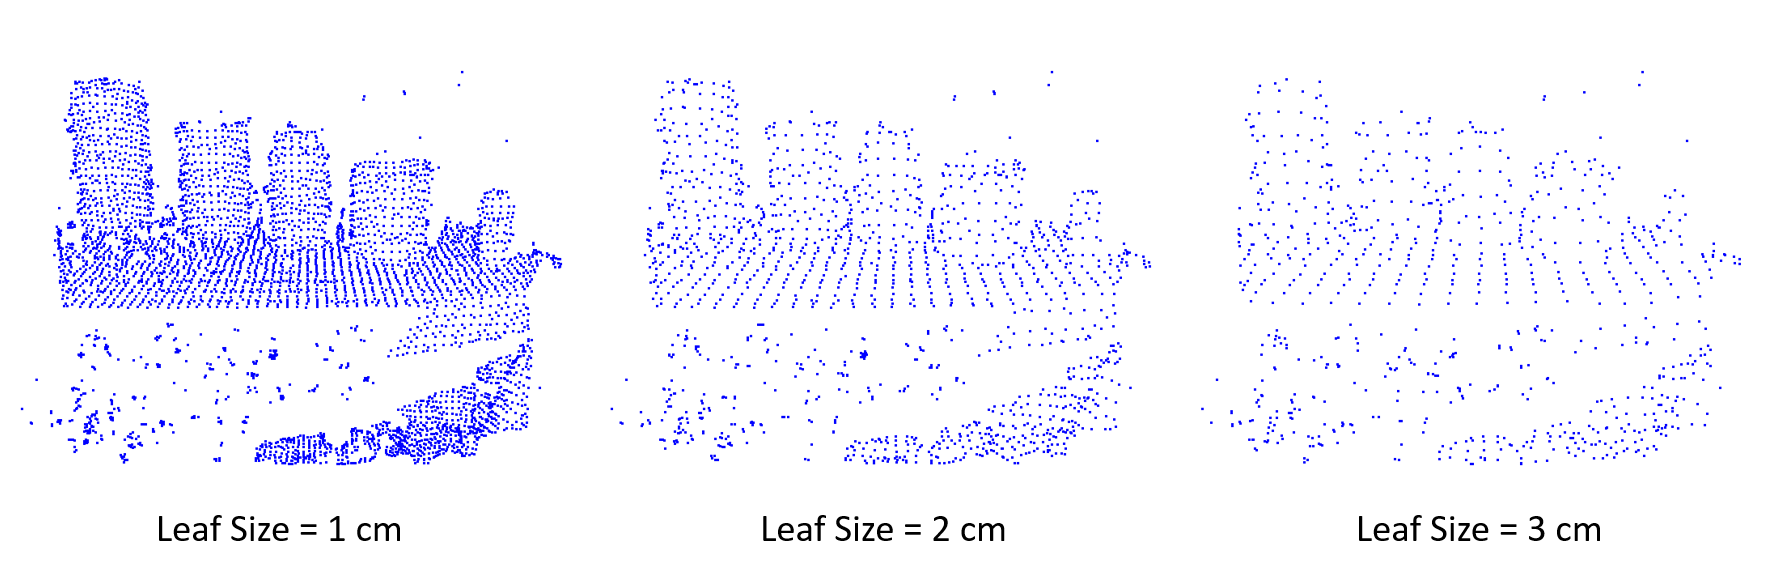
\includegraphics[width=\textwidth]{images/image11}
  \caption{Downsampling results for several different leaf sizes.}
\end{figure*}
\begin{figure*}
  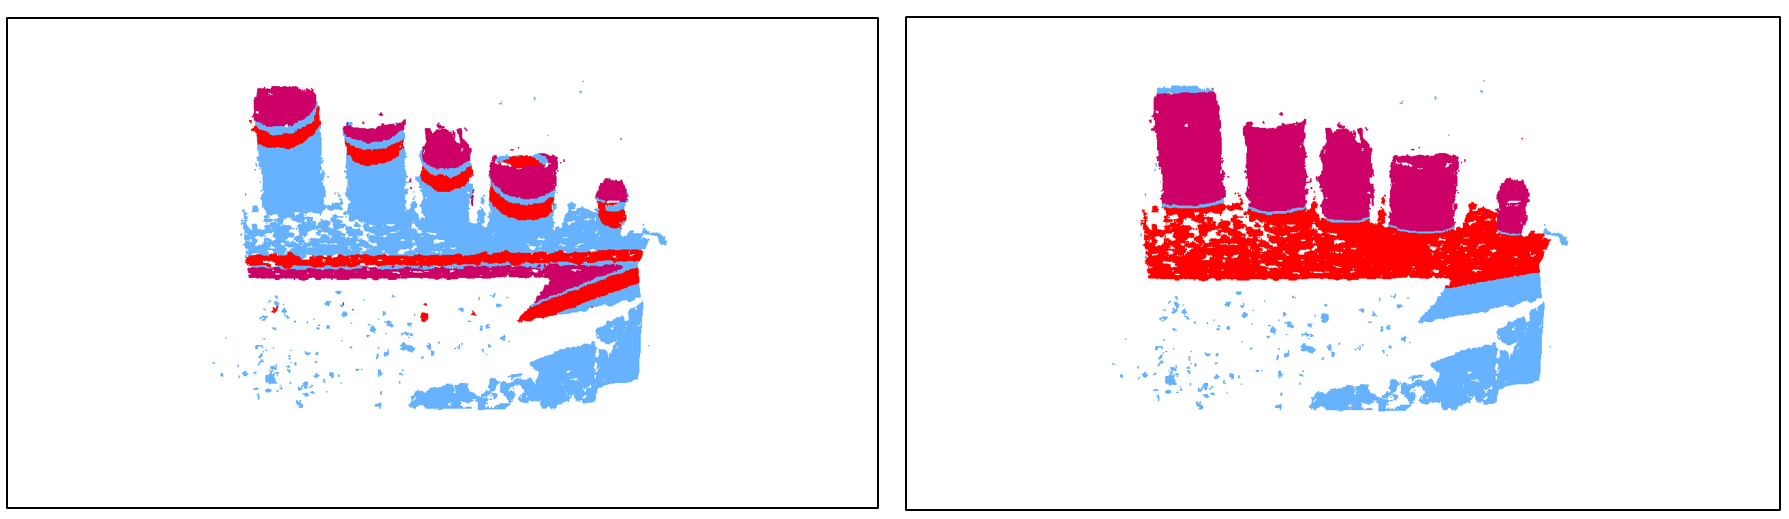
\includegraphics[width=\textwidth]{images/image06-notext}
  \caption{The effects of varying the number of iterations of RANSAC.  Notice that the plane on the left, which only used 200 iterations, was not correctly identified, while the one on the right, with 600 iterations was correctly identified.}
\end{figure*}

\subsection{Plane/Prism Extraction and the RANSAC Algorithm}

RANSAC is a quick method of finding mathematical models.  In the case of a plane, the RANSAC method will create a virtual plane that is then rotated and translated throughout the scene looking for the plane with the data points that fit the model (aka., Inliers).  The two parameters used are the threshold distance and the number of iterations.  The greater the threshold, the thicker the plane can be.  The more iteration RANSAC is allowed to do, the greater the probability of finding the plane with the most inliers.  In Fig. 2, one can see what happens as the number of iterations is changed.  The blue points represent the original data, the red points represent the plane inliers, and the magenta points represent the noise (aka. Outliers) remaining after prism extraction.  As can be seen, the image on the left shows how the plane of the table was not found due to RANSAC not being given enough iterations.  The image on the right shows the plane being found and the objects above the plane being properly segmented from the original data. 


\subsection{Clustering}
The last stage in the segmentation process is Euclidean clustering. This process takes the down sampled point cloud, without the plane and its convex hull, and breaks it into clusters, with each cluster hopefully corresponding to one of the objects on the table.  This is accomplished by first creating a kd-tree data structure, which stores the remaining points in the cloud in a way that can be searched efficiently, and then the cloud points are iterated over, with a radius search being performed for each point. Neighboring points within the threshold radius are then added to the current cluster, and marked as processed.  This continues until all points in the cloud have been marked as processed. When the algorithm terminates, all the points in the cloud have been put into different segments.



\section{The Object Recognition Pipeline}
The goal of object recognition is to pick out some object of interest from the scene, in order to get the information about its position and orientation. For our research, we are interested in identifying the position of the robot hand at a particular instant of time so that the robot hand can be guided to pick up the segmented object. This requires having a model of the robot hand in order to compare it against the objects in the scene.  

There are  two standard approaches in 3D object recognition to compare the model and the scene: the 1global pipeline and local pipeline. As shown in Fig. 3, these two techniques achieve the goal of object comparison/matching through the implementation of two distinct sequences (pipelines) of feature recognition algorithms. Particularly, they use different descriptors to compare the objects. A descriptor encodes information on model and scene images to make it possible to compare them. 
Next, we give a description of the global and local approaches to object recognition .
\subsection{The Global Approach}
The global pipeline works by taking the object clusters from the earlier clustering step and computing a histogram for each of them.  This histogram is then compared against a database of pre-calculated histograms for some object of interest, in our case, the robot's hand.  These pre-calculated histograms are simply loaded at program boot-time.  There are many histograms in the database for each object of interest because one needs to have data representing an object from many different camera positions.

There are several global descriptors that are available to store the data: Viewpoint Feature Histogram (VFH), Clustered Viewpoint Feature Histogram (CVFH), Oriented, Unique and Repeatable CVFH (OUR-CVFH), Ensemble of Shape Functions (ESF), and the Global Radius-based Surface Descriptor (GRSD).  All of these variants were tested by our group, but we ended up choosing the OUR-CVFH descriptor, mainly because that was the approach favored by some of the original authors of PCL \cite{aldoma4}.


\subsubsection{VFH}
The VFH has a viewpoint dependent part, which stores data on the angles between the normal vectors of the points in the cloud and the vector from the camera viewpoint to the cluster centroid.  Another portion of the histogram stores data on the distances of the points in the cluster to the cluster’s centroid.  There are other components to the histogram as well, but the full details are somewhat beyond the scope of this handout, and the reader is referred to \cite{clusterrec} for a detailed description. 

\subsubsection{CVFH}
The Clustered VFH descriptor is similar to VFH except that it first divides the cluster into several regions using region-growing segmentation.  An example would be a milk carton being divided into clusters corresponding to the sides of the carton.  From here, VFHs are computed for each region.  This offers an  advantage over VFH, in that only one of the regions needs to be visible for the object to be identified.  So, for example, if the desired object is occluded by some other object standing in front of it, the desired object can still be picked out based on the visible part.
\begin{figure*}
  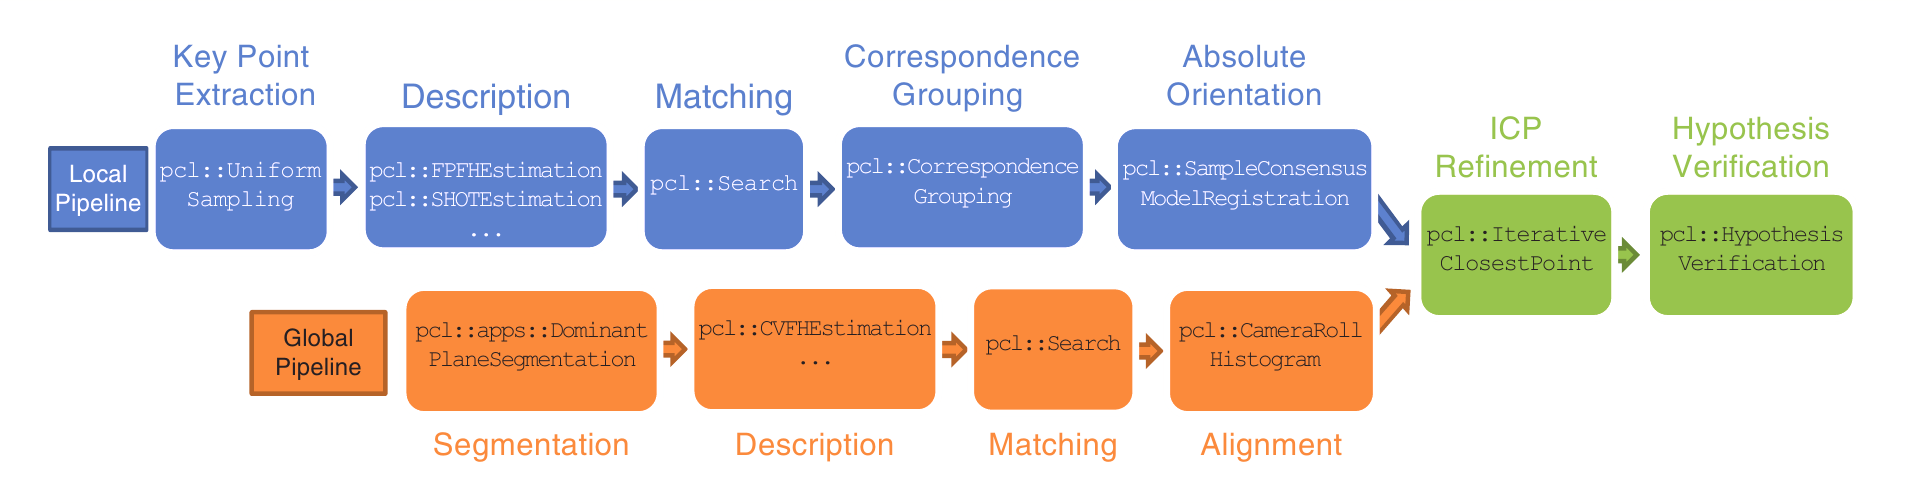
\includegraphics[width=\textwidth]{images/image12}
  \caption{The 2 approaches to object recognition: local pipeline (top) and global pipeline (bottom).  Image taken from \cite{aldoma2} }
\end{figure*}

\subsubsection{OUR-CVFH}
The Oriented, Unique, Repeatable CVFH descriptor extends CVFH by adding one additional processing stage after the region segmentation.  It further filters the points in each region according to their difference from the region’s average normal, thereby refining knowledge of the region’s shape.  
	After this step, a Semi-Global Unique Reference Frame (SGURF), aka, a local coordinate system, is computed for each region.  It is these reference frames which make up the content of the descriptor.  The full detail of this process can be found in \cite{aldoma4}. 
	The result of these extra processing phases is an 82\% detection rate which is a notable improvement over other global descriptors.\cite{aldoma4}
	
\subsection{The Local Approach}
Local object recognition techniques extract key point information in the model and the scene images and associate them to a local 3D descriptor neighborhood \cite{aldoma}. Local keypoints provide information on the local geometric features such as image position and coverage area. A local descriptor compares the keypoints between the model and the scene. Unlike global descriptors that describe an entire object, local descriptors use multiple points in the image for comparison. Since the local feature recognition technique can operate on image patches, it gives promising recognition even for occluded and cluttered scenes in which the global feature recognition technique fails.

In order to quantify the performance of the local pipeline relative to the global pipeline, we evaluated the correspondence grouping and object alignment techniques which are based on local feature descriptors \cite{aligning} \cite{aldoma3}.  In each of the pipelines, we first downsample the point cloud, and then take the keypoints associated with  them.  We then use the keypoints to create 3D local descriptors, namely Signature of Histograms of Orientations (SHOT) and Fast Point Feature Histogram (FPFH). After this, matching is performed to determine the presence of model instances in the scene.
Although we were able to achieve high accuracy of object recognition using local pipelines, its computation time was higher than our execution time requirement, hence we abandoned this approach.

\section{Bounding Box}
After the object segmentation and recognition has been performed, the robot knows which object to pick up, but it doesn't know the boundaries of the object. The boundary of the object is supplied by creating a rectangular bounding box around the object.  This is the final stage in the task of segmenting a single frame of depth imagery.  Next we present the steps taken in the bounding box calculation.

 \begin{enumerate}
	\item[1.] Compute mean value vector of the points in the cloud, call it $\overline{p}$
\begin{equation}
\overline{p} =\left(\frac{\sum p_x}{\text{points.size}}, \frac{\sum p_y}{\text{points.size}},\frac{\sum p_z}{\text{points.size}}\right)
%\left(
%\begin{matrix}
%	\frac{\sum p_x}{\text{points.size}} \\ \\
%	\frac{\sum p_y}{\text{points.size}}\\ \\
%	\frac{\sum p_z}{\text{points.size}}	
%\end{matrix}	
%\right)
\end{equation}
\item[2.] Compute the covariance matrix, $M_{\text{cov}}$
\begin{align}
M_{\text{cov}} &= \sum_{p \, \in \, \text{points}} 
	\left(
\begin{array}{c}
p_x\\
p_y\\
p_z\\
\end{array}
\right)
\left(
\begin{matrix}
p_x & p_y & p_z	
\end{matrix}
\right)\\ &= \sum_{p \, \in \, \text{points}}
\left(
\begin{matrix}
	p_x p_x & p_x p_y & p_x p_z \\
	p_x p_y & p_y p_y & p_y p_z \\
	p_x p_z & p_y p_z & p_z p_z
\end{matrix}
\right)
\end{align}
\item[3.] Solve for the eigenvectors and eigenvalues of the covariance matrix.  The three eigenvectors --- major, middle, and minor --- then make up the columns, aka., the axes, of the rotation matrix
\begin{align}
	M_\text{rot} = 
	\left(
	\begin{matrix}
		\text{major}_x & \text{middle}_x & \text{minor}_x\\
		\text{major}_y & \text{middle}_y & \text{minor}_y\\
		\text{major}_z & \text{middle}_z & \text{minor}_z
	\end{matrix}
	\right)
\end{align}
\item[4.] Compute the max and min points for the bounding box: for every point $p$ in the cloud, compute the difference from the mean value vector, rotated by the rotation matrix, i.e.,
\begin{align}
	p^{\prime} = M_{\text{rot}}^T (p - \overline{p})
\end{align}
which is equivalent to,
\begin{align}
	p_x^{\prime} = (p - \overline{p}) \cdot (\text{major\_axis})\\
	p_y^{\prime} = (p - \overline{p}) \cdot (\text{middle\_axis})\\
	p_z^{\prime} = (p - \overline{p}) \cdot (\text{minor\_axis})
\end{align}
and then compare these to the current max/min point values.  If they are greater or lesser respectively, then overwrite them with these new values.
\item[5.] Compute the midpoint between the max and min points.  This is the shift vector.
\begin{align}
	\text{shift} = 	\frac{\text{max\_point} + \text{min\_point}}{2}
\end{align}
Adjust the max/min points by the shift, as well as setting the position vector to the center of the box
\begin{align}
	p_{\text{max}} = p_{\text{max}} - \text{shift} \\ p_{\text{min}} = p_{\text{min}} - \text{shift}\\ p_{\text{cm}} = \overline{p} + (M_{\text{rot}})( \text{shift})
\end{align}





\end{enumerate}
The bounding box is completely described by the rotation matrix, center of mass, and max and min points.  This gives the robot everything it needs to pick the object of interest.
\begin{figure*}
\begin{tabular}{cc}
  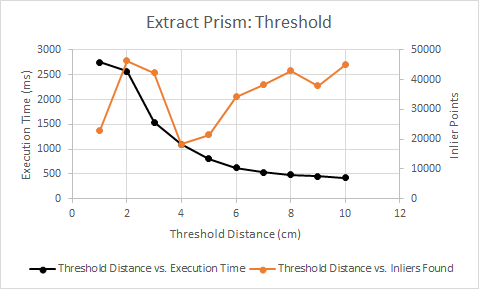
\includegraphics[width=0.5\textwidth]{images/image00} &   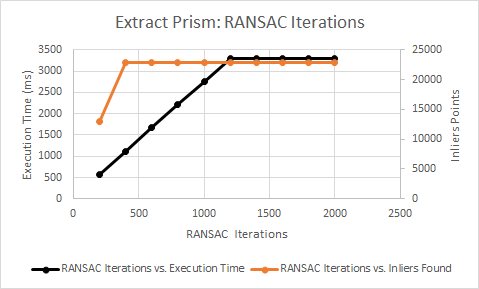
\includegraphics[width=0.5\textwidth]{images/image09} \\
(a) & (b) \\[6pt]
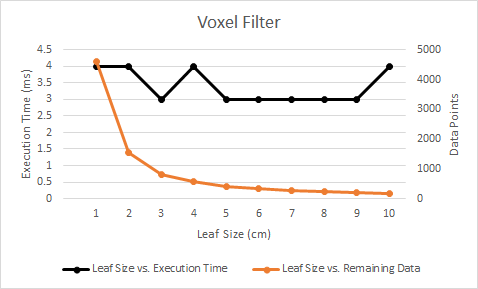
\includegraphics[width=0.5\textwidth]{images/image08} & 
 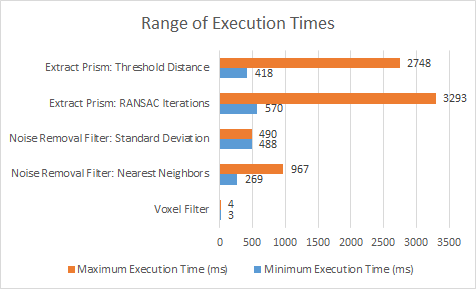
\includegraphics[width=0.5\textwidth]{images/image05} \\
(c) & (d) \\[6pt]


\end{tabular}
\caption{Comparison of the effects of various parameters on segmentation pipeline performance}
\end{figure*}

\section{Testing}
To test the performance of the segmentation pipeline, we first needed to find the effect of each function parameter on the execution time of the program.  To do this, the program was run by only changing one parameter at a time over a range of values.  As shown in Figure 4 (bottom-right), not all functions in the segmentation pipeline have an equal impact on the execution time.  This led to some functions being optimized for performance over the resulting point cloud data.

The images in Figure 4 further show the results of each individual test.  All parameters, with the exception of the one being tested, were held constant for each test.  Also, the source point cloud data used was a raw unmodified image from the Realsense camera.  For each graph, the dark line represents the execution time in comparison to the parameter being tested.  The lighter (orange) line shows how many points are left in the resulting PCD file.

\section{Applications}
There are several practical applications of object segmentation. Machine vision, medical imaging, human machine interaction, place recognition, object detection, video surveillance and manufacturing industry are some of the fields where our object segmentation and recognition package could be useful.
\section{Future Work}
\subsection{Accuracy Benchmarking}
We also researched a method for measuring the accuracy of bounding boxes calculated by our segmentation pipeline.  In this method an image is first analyzed without downsampling so that the resulting bounding box is regarded as an ideal model. Then, the segmentation parameters can be adjusted and the degradation in accuracy caused by these adjustments can be measured quantitatively.

The first step in the process is to find the best fit pairing between the corners of the cube.  This is done by comparing, pointwise, all possible corner matchings, and calculating their distances 

Once this best fit matching of the corners has been obtained, we can calculate the accuracy of a box with respect to the ideal box-model.  This calculation was motivated with the following reasoning. A corner of the box is defined to be 100\% accurate if it has the exact position of the corner in the box which is being compared, and the accuracy will fall off exponentially as the distance between the corners increases, reaching zero if the distance between them is infinity.  So, it is reasonable to say that the accuracy will be halved for each unit of distance between the 2 corners.  This distance unit should be chosen based on the context.  For example, if the application is dealing with small objects, a distance unit of a few centimeters might be appropriate.  Since there are 8 corners to compare between the 2 bounding boxes, the total accuracy will be the geometric mean of the product of the accuracies for the 8 corners.  



Symbolically, this is the quantitative definition of accuracy in the context of comparing boxes:
\begin{figure}
  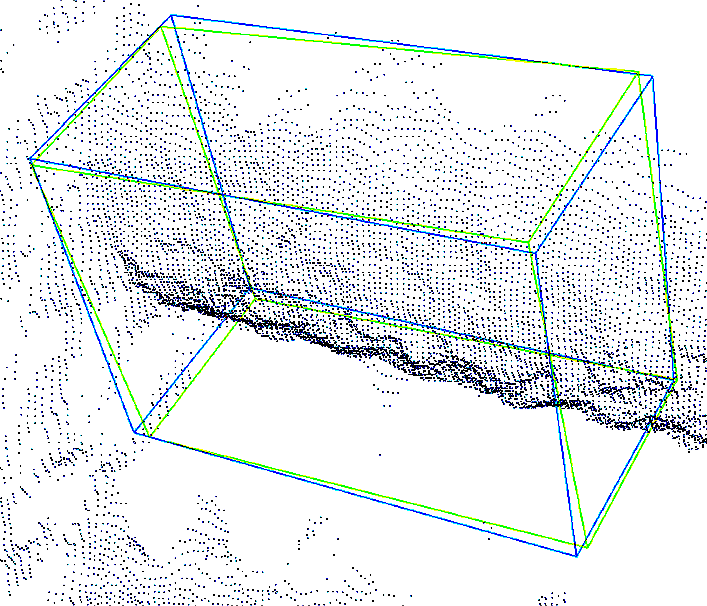
\includegraphics[scale=0.35]{images/accuracy-image-inverted}
  \caption{Bounding box accuracy demo, showing two boxes which agree to 95\% accuracy.}
\end{figure}


\begin{equation}
	 \text{accuracy} \equiv \sqrt[8]{\prod_{i=1}^{8} 2^{-sd_i}}
\end{equation}
where $d_i$ is the distance between the i'th corner in the first box, and the i'th corner in the second box, which is given by the standard Euclidean distance formula:\\
\begin{equation}
	d_i = \sqrt{(x_{1_i} - x_{2_i})^2 + (y_{1_i} - y_{2_i})^2 + (z_{1_i} - z_{2_i})^2}\\
\end{equation}

This algorithm has been implemented in our code base, but it took second priority to getting the segmentation pipeline working, and for that reason has not been extensively tested.

\subsection{GPU Support}The next thing we could improve on would be to add GPU support, e.g., Nvidia's CUDA, which could greatly increase performance.  GPU support comes as a part of PCL, but is disabled by default.  Therefore, the only cost of adding this feature would be to determine the necessary compiler flags and changes to the build process.

\subsection{Machine Learning}Another feature we would like to explore further is some kind of machine learning, aka, self-tuning capability.  If the pipeline were able to adjust its parameters based on environmental conditions, it could be a lot more robust.  For example, if the table surface was not very reflective, which tends to make plane extraction fraught with difficulty, the adaptive pipeline could increase the number of RANSAC iterations in order to correctly identify the plane.  We have done some work implementing a genetic algorithm for this purpose; however, further work is necessary before it can be incorporated into the pipeline. 

\section{Conclusion}
We were able to successfully implement an object segmentation pipeline and an object recognition pipeline, achieving a frame rate between 2-4 frames per second.  We have provided our code as a ROS node which is freely available on github \cite{c44source} under the BSD license, so that future users are free to build on our results.



\begin{thebibliography}{1}

\bibitem{aldoma4}
Aldoma, Aitor et al. "OUR-CVFH – Oriented, Unique and Repeatable Clustered Viewpoint Feature Histogram for Object Recognition and 6DOF Pose Estimation."  Computer Vision Laboratory, Dept. of Computer Science and Engineering, University of Bologna.  Accessed June 2, 2016.  http://vision.deis.unibo.it/fede/papers/dagm12.pdf

\bibitem{clusterrec}
"Cluster Recognition and 6DOF Pose Estimation using VFH descriptors." \emph{pointclouds.org}.  Perception Foundation.
Accessed May 29, 2015. http://pointclouds.org/documentation/tutorials/vfh\_recognition.php



\bibitem{aldoma2}
Aldoma, Aitor et al.  "Three-Dimensional Object Recognition and 6 DoF Pose Estimation." \emph{IEEE Robotics \& Automation Magazine}, September 2012.


\bibitem{aldoma}
Aldoma, Aitor, Federico Tombari, Luigi Di Stefano, and Markus Vincze, "A global hypotheses verification method for 3D object recognition.," In \emph{Computer Vision-ECCV}, pp. 511-524. Springer Berlin Heidelberg, 2012.

\bibitem{aligning}
"Aligning Object Templates to a Point Cloud." - Point Cloud Library (PCL).  Accessed May 30, 2016.  http://pointclouds.org/documentation/tutorials/template\_alignment.php.


\bibitem{aldoma3}
Aldoma, Aitor, and Federico Tombari. "3D Object Recognition Based on Correspondence Grouping." - Point Cloud Library (PCL). Accessed May 30, 2016. http://www.pointclouds.org/documentation \\ /tutorials/correspondence\_grouping.php. 


\bibitem{6DOF}
"PCL/OpenNI tutorial 5: 3D object recognition (pipeline)." Robotics Group of the University of Leon.  Updated Nov 1, 2015.  Accessed May 29, 2015.  http://robotica.unileon.es/mediawiki/index.php \\ /PCL/OpenNI\_tutorial\_5:\_3D\_object\_recognition\_(pipeline).


\bibitem{c44source}
"Object Vision 3D" source code: https://github.com/j1mb0/object\_vision\_3D
\end{thebibliography}

 % You can push biographies down or up by placing
% a \vfill before or after them. The appropriate
% use of \vfill depends on what kind of text is
% on the last page and whether or not the columns
% are being equalized.

%\vfill

% Can be used to pull up biographies so that the bottom of the last one
% is flush with the other column.
%\enlargethispage{-5in}



% that's all folks
\end{document}


